\chapter{Software}
\vspace{-19mm}
The STM microcontroller has an ARM Cortex-32-bit RISC core that will be programmed in C using Atollic TrueSTUDIO. The IDE will compile and upload the code to the STM using the ST-link debugger and toolchain. All code can be found in the GitHub repository. \textbf{https://github.com/Marshmellowfellow/Thesis-Servocontroller-Board.git}
\vspace{-12mm}

\section{ADC}
\vspace{-8mm}

\begin{table}[H]
\centering
    \begin{tabular}{|l|l|}
    \hline
            \textbf{\underline{Initialisations:}}&\textbf{\underline{Main:}}\\
            1. Configure GPIO pins & 1. Select channel to sample\\
            2. Enable ADC clock    & 2. Activate ADC to be read\\
            3. Set ADC parameters  & 3. Start conversion\\
                                   & 4. Read in ADC value\\
                                  \hline
    \end{tabular}
    \caption{ADC code implementation}
\end{table}

\vspace{-12mm}
\subsection{Testing}
\vspace{-7mm}
In order to test the implementation of the ADC code a voltage in the range 0V-3V will be applied to the ADC pin of the micro controller. The ADC will sample with an 8-bit resolution. This will give $\mathbf{2^8 - 1 = 255}$ bits, giving a resolution of $\mathbf{\frac{3}{255}\frac{V}{Steps}}$ = $\mathbf{11.76\frac{mV}{step}}$. 
\vspace{-9mm}

The ADC will store an 8-bit value representing the sampled input into the ADC Data Register(DR). This value will then be written to the General Purpose Input Output(GPIO) Output Data Register(ODR). GPIO pins 0-7 will be set in output mode and connected to an LED. The binary value of the sample can then be output to the 8-bit LED output so that it can be read and compared to the actual voltage at the ADC input pin. 

\vspace{-2mm}
The binary value output will be a number between 0-255. The voltage calculated using $V_{calculated} = (ADC_{output})\times(resolution) $. The applied voltages and sampled values can be seen below in ..table.. and were calculates using the resolution of $11.76\frac{mV}{step}$ 

\begin{table}[H]
\vspace{-2mm}
    \centering
    \begin{tabular}{ |c| c| c| }
        \hline
         \textbf{\underline{$\mathbf{V_{Applied}}$} (V)} & \textbf{\underline{Output 8-bit value}} & \textbf{\underline{$V{Calculated}$ (V)}} \\
         0.66 & 00110000 & 564.48 \\
         1.21 & 01011000 & 1.03 \\
         1.81 & 10000100 & 1.55 \\
         2.36 & 10101100 & 2.02 \\
         3.30 & 11111110 & 2.99 \\
         \hline
    \end{tabular}
    \vspace{-2mm}
    \caption{ADC testing applied voltages}
    \vspace{-3mm}
\end{table}
\vspace{-8mm}
It can be seen that with some error, the ADC was cable of sampling a voltage. Thus the microcontroller can read an output voltage from the current and temperature sensors.


\newpage
\section{PWM}
\vspace{-3mm}
The following configurations were implemented in order to output a PWM signal at a GPIO pin.

\begin{table}[H]
\centering
    \begin{tabular}{|l|l|}
    \hline
            \textbf{\underline{Initialisations:}}&\\
            1. Enable the GPIO clock        & 6. Set timer to PWM mode 1\\
            2. Enable the timer             & 7. Set signal frequency\\
            3. Set GPIO pins to AF          & 8. Set duty cycle\\
            4. Map GPIO pins to the timer   & 9. Enable output compare\\
            5. Map GPIO pins to the timer   & \\
                                  \hline
    \end{tabular}
    \caption{PWM initialisations}
\end{table}

\subsection{Testing}
\vspace{-5mm}
The PWM configuration was tested by outputting a PWM signal and connecting to an oscilloscope.

\begin{figure}[H]
    \centering
    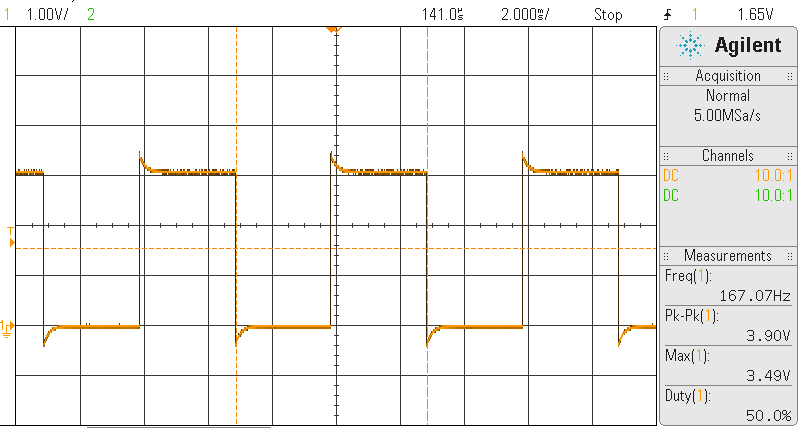
\includegraphics[width=1\textwidth]{pwm.png}
    \vspace{-5mm}
    \caption{Oscilloscope output}
\end{figure}
\vspace{-5mm}
It can be seen that a PWM signal with a 50\% duty cycle was successfully implemented and is cable of control the servomotors position through varying the Duty Cycle of the signal.

\newpage
\section{USART}

\begin{table}[H]
\centering
    \begin{tabular}{|l|l|}
    \hline
            \textbf{\underline{Initialisations:}}&\textbf{\underline{Implementation:}}\\
            1. Enable the UART clock        & \textbf{Transmit}\\
            2. Enable the GPIO clock        & 1. Write data to USART TDR\\
            3. Set GPIO pins to AF          & 2. Store message into a variable\\
            4. Clear USART control register & 3. Clear USART ICR\\
            5. Define clock speed           & \textbf{Receive}\\
            6. Set baud rate and parity     & 1. Wait for Message\\
            7. Enable USART TX and RX       & 2. Store message into a variable\\
                                            & 3. Clear USART ICR\\
                                  \hline
    \end{tabular}\
    \vspace{-2mm}
    \caption{USART initialisations and implementation}
\end{table}


\vspace{-8mm}
\subsection{Testing}
\vspace{-7mm}
\subsubsection{Transmit}
\vspace{-7mm}
The microcontroller was programmed to transmit the three messages "0000000", "1101011", "0000000" every 10 mili seconds using the serial protocol. The TX pin was probed with an oscilloscope and the transmitted message can be seen below in Figure 7.2 The "1's" represented by 3.3V and "0's" by 0V.

\begin{figure}[H]
\centering
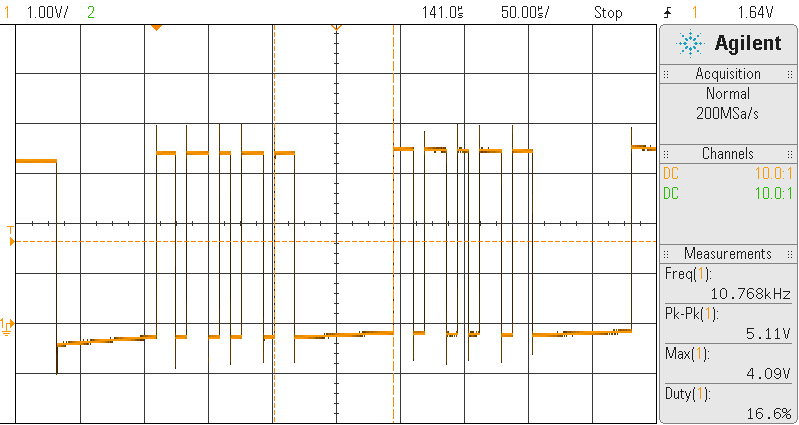
\includegraphics[width=0.8\textwidth]{rs485.png}
\vspace{-6mm}
\caption{Oscilloscope output}
\vspace{-10mm}
\end{figure}
\subsubsection{Receive}
\vspace{-9mm}
A master microcontroller was programmed to transmit the three messages "0000000", "1101011", "0000000" every 100 mili seconds using the serial protocol. A slave was then made to receive the message and display the 8-bit output on 8 LED's to be compared to the 8-bit message sent. The implementation worked as designed.

\newpage
\section{Final code implementation}

\begin{table}[H]
\centering
    \begin{tabular}{|l|l|}
    \hline
            \textbf{\underline{Initialisations:}}&\textbf{\underline{Initialisations:}}\\
            &\\
            1. GPIO pins for LED's and switches & 1. GPIO pins for LED's and switches\\
            &\\
            2. USART             & 2. USART\\
            3. PWM               & 3. PWM\\
            4. ADC               & 4. ADC\\
            &\\
            \textbf{Main:}                             &  \textbf{Main:}\\
            1. Check for button press                  & 1. Check for button press\\
            2. Read in voltage from potentiometer      & 2. Transmit message to master with USART\\
            3. Transmit message to slave with USART    & 3. Wait for USART message from master\\
            4. Wait for USART message from slave       & 4. Output PWM signal to servomotor\\
            5. Control status LED                      & 5. Control status LED \\
                                                       & 6. Read in current and temperature sensors \\
                                  \hline
    \end{tabular}\
    \vspace{-2mm}
    \caption{Final initialisations and implementation}
\end{table}
